% Figure 1: CoupleFlow architecture. Thumbnails: tools/unified/fig_architecture.py.
% Colours: blue = neural path, orange = acoustic path, green = coupling/decoding,
% pink = flow (density), gold = anti-shortcut, grey = auxiliary.
\definecolor{cfN}{HTML}{2A78D6}\definecolor{cfA}{HTML}{EB6834}
\definecolor{cfC}{HTML}{1BAF7A}\definecolor{cfF}{HTML}{D6558A}
\definecolor{cfG}{HTML}{C98A00}\definecolor{cfX}{HTML}{7A7974}
\begin{tikzpicture}[x=1cm,y=1cm,>={Stealth[length=4.5pt,width=3.6pt]},
  blk/.style 2 args={draw=#1,fill=#1!6,rounded corners=3pt,line width=0.75pt,align=center,
    inner sep=2pt,font=\scriptsize,minimum width=#2cm,minimum height=1.1cm},
  emb/.style={draw=#1,fill=#1!14,rounded corners=3pt,line width=0.75pt,align=center,
    inner sep=2pt,font=\scriptsize,minimum width=1.75cm,minimum height=0.8cm},
  loss/.style={draw=#1,fill=#1!16,rounded corners=5pt,line width=0.5pt,inner sep=1.8pt,
    font=\scriptsize},
  fl/.style={->,line width=0.8pt,draw=#1},
  tie/.style={line width=0.55pt,draw=#1,densely dotted},
  lab/.style={font=\scriptsize,text=black!75}]
\providecommand{\cfttl}[1]{\textbf{#1}\\[1pt]}

% ------------------------------------------------------------------ inputs
\node[inner sep=0] (eeg) at (1.00,4.40) {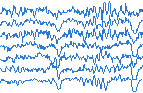
\includegraphics[width=2.0cm,height=1.25cm]{figures/arch_eeg.pdf}};
\node[lab,above=3pt of eeg] {EEG $x\in\mathbb{R}^{C\times L}$};
\node[inner sep=0] (env) at (1.00,0.80) {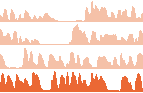
\includegraphics[width=2.0cm,height=1.25cm]{figures/arch_env.pdf}};
\node[lab,below=3pt of env] {envelopes $a_1,\dots,a_K$};

% ------------------------------------------------------------------ neural row
\node[blk={cfN}{2.7}] (lc) at (3.75,4.40)
  {\cfttl{Listener correction}$x\mapsto x+U_m V_m^{\top}x$\\ rank 2, listener $m$};
\node[blk={cfN}{2.1}] (vs) at (6.70,4.40) {\cfttl{Virtual sensors}$1{\times}1$ conv, $C\to8$};
\node[blk={cfN}{3.0}] (enc) at (9.85,4.40)
  {\cfttl{Lag-window encoder}5 dilated convs; $e_t$ sees\\
   EEG in $[t{+}\delta,\ t{+}\delta{+}0.98\,\mathrm{s}]$};
\node[emb=cfN] (e) at (12.85,4.40) {neural emb.\\ $e\in\mathbb{R}^{16\times L}$};
\draw[fl=cfN] (eeg.east) -- (lc.west);
\draw[fl=cfN] (lc.east) -- (vs.west);
\draw[fl=cfN] (vs.east) -- (enc.west);
\draw[fl=cfN] (enc.east) -- (e.west);

% ------------------------------------------------------------------ acoustic row
\node[blk={cfA}{2.7}] (feat) at (3.75,0.80)
  {\cfttl{Candidate features}envelope, onsets,\\ sub-bands, glimpses};
\node[blk={cfA}{2.1}] (qm) at (6.70,0.80) {\cfttl{Quantile match}equal envelope\\ distributions};
\node[blk={cfA}{3.0}] (aenc) at (9.85,0.80)
  {\cfttl{Shared encoder}causal dilated convs,\\ same weights for all $k$};
\node[emb=cfA] (ah) at (12.85,0.80) {cand.\ emb.\\ $\hat{a}_k\in\mathbb{R}^{16\times L}$};
\draw[fl=cfA] (env.east) -- (feat.west);
\draw[fl=cfA] (feat.east) -- (qm.west);
\draw[fl=cfA] (qm.east) -- (aenc.west);
\draw[fl=cfA] (aenc.east) -- (ah.west);

% ------------------------------------------------------------------ flow head (middle left)
\node[blk={cfF}{7.6},minimum height=1.05cm] (flow) at (6.45,2.60)
  {\cfttl{Flow head: conditional flow matching on the envelope}
   residuals $R_{\rm cond}(a_k)$, $R_{\rm unc}(a_k)$ with / without $e$\\
   PMI rule: $\arg\max_k\,[R_{\rm unc}-R_{\rm cond}](a_k)$};
\draw[fl=cfA] (env.north) |- (flow.west) node[pos=0.3,left,lab] {$a_k$};
\draw[fl=cfN] ([xshift=3mm]enc.south) -- ([xshift=3mm]enc.south|-flow.north)
  node[midway,right,lab] {$e$};
\node[loss=cfF,anchor=south west] (Lfm) at ([xshift=2mm,yshift=1.5pt]flow.north west) {$\mathcal L_{\rm FM}$};

% ------------------------------------------------------------------ coupling + decision (middle right)
\node[blk={cfC}{3.6},line width=1pt,minimum height=1.05cm] (cs) at (12.85,2.60)
  {\cfttl{Time-centred coupling}$s(e,\hat a_k)={}$\\$\frac{1}{\tau}\sum_{d}\omega_d\,\mathrm{corr}_t(e_d,\hat a_{k,d})$};
\draw[fl=cfN] (e.south) -- (cs.north);
\draw[fl=cfA] (ah.north) -- (cs.south);
\node[blk={cfC}{2.1},line width=1pt,minimum height=1.05cm] (dec) at (16.35,2.60)
  {\cfttl{Decision}$\hat y=\arg\max_k s_k$};
\draw[fl=cfC] (cs.east) -- (dec.west);

% ------------------------------------------------------------------ losses (tags)
\node[loss=cfX] (Lside) at (4.80,5.55) {$\mathcal L_{\rm side}$: side head (training only)};
\draw[tie=cfX] (Lside.south-|lc.north) -- (lc.north);
\node[loss=cfG,anchor=east] (Lvic) at (12.75,5.55) {$\mathcal L_{\rm VIC}$};
\node[loss=cfX,anchor=west] (Lenv) at (12.95,5.55) {$\mathcal L_{\rm env}$};
\draw[tie=cfG] (Lvic.south) -- ([xshift=-3mm]e.north);
\draw[tie=cfX] (Lenv.south) -- ([xshift=3mm]e.north);
\node[loss=cfC,anchor=east] (Lce) at (16.25,3.75) {$\mathcal L_{\rm CE}$};
\node[loss=cfC,anchor=west] (Lnce) at (16.45,3.75) {$\mathcal L_{\rm NCE}$};
\draw[tie=cfC] (Lce.south) -- (Lce.south|-dec.north);
\draw[tie=cfC] (Lnce.south) -- (Lnce.south|-dec.north);
\node[loss=cfG] (Lnull) at (16.35,1.50) {$\mathcal L_{\rm null}$};
\draw[tie=cfG] (Lnull.north) -- (dec.south);
\node[loss=cfG,anchor=west] (Ladv) at (14.20,0.80) {$\mathcal L_{\rm adv}$: audio-only classifier};
\draw[tie=cfG] (ah.east) -- (Ladv.west);
\draw[->,line width=0.65pt,draw=cfG,dashed] (ah.south) -- ++(0,-0.42) -| (aenc.south)
  node[pos=0.25,below,lab] {reversed gradient};
\end{tikzpicture}
